\AtBeginSection[]{
    \begin{frame}
        \frametitle{}
        \tableofcontents[currentsection]
    \end{frame}
}

%%%%%%%%%%%%%%%%%%%%%%%%%%%%%%%%%%%%

\section{Theoretical background}

\subsection{Multi-Agent Systems context}

\begin{frame}{Theoretical background}{Organizational model: $\mathcal{M}OISE^+$}

    \begin{figure}
        \centering
        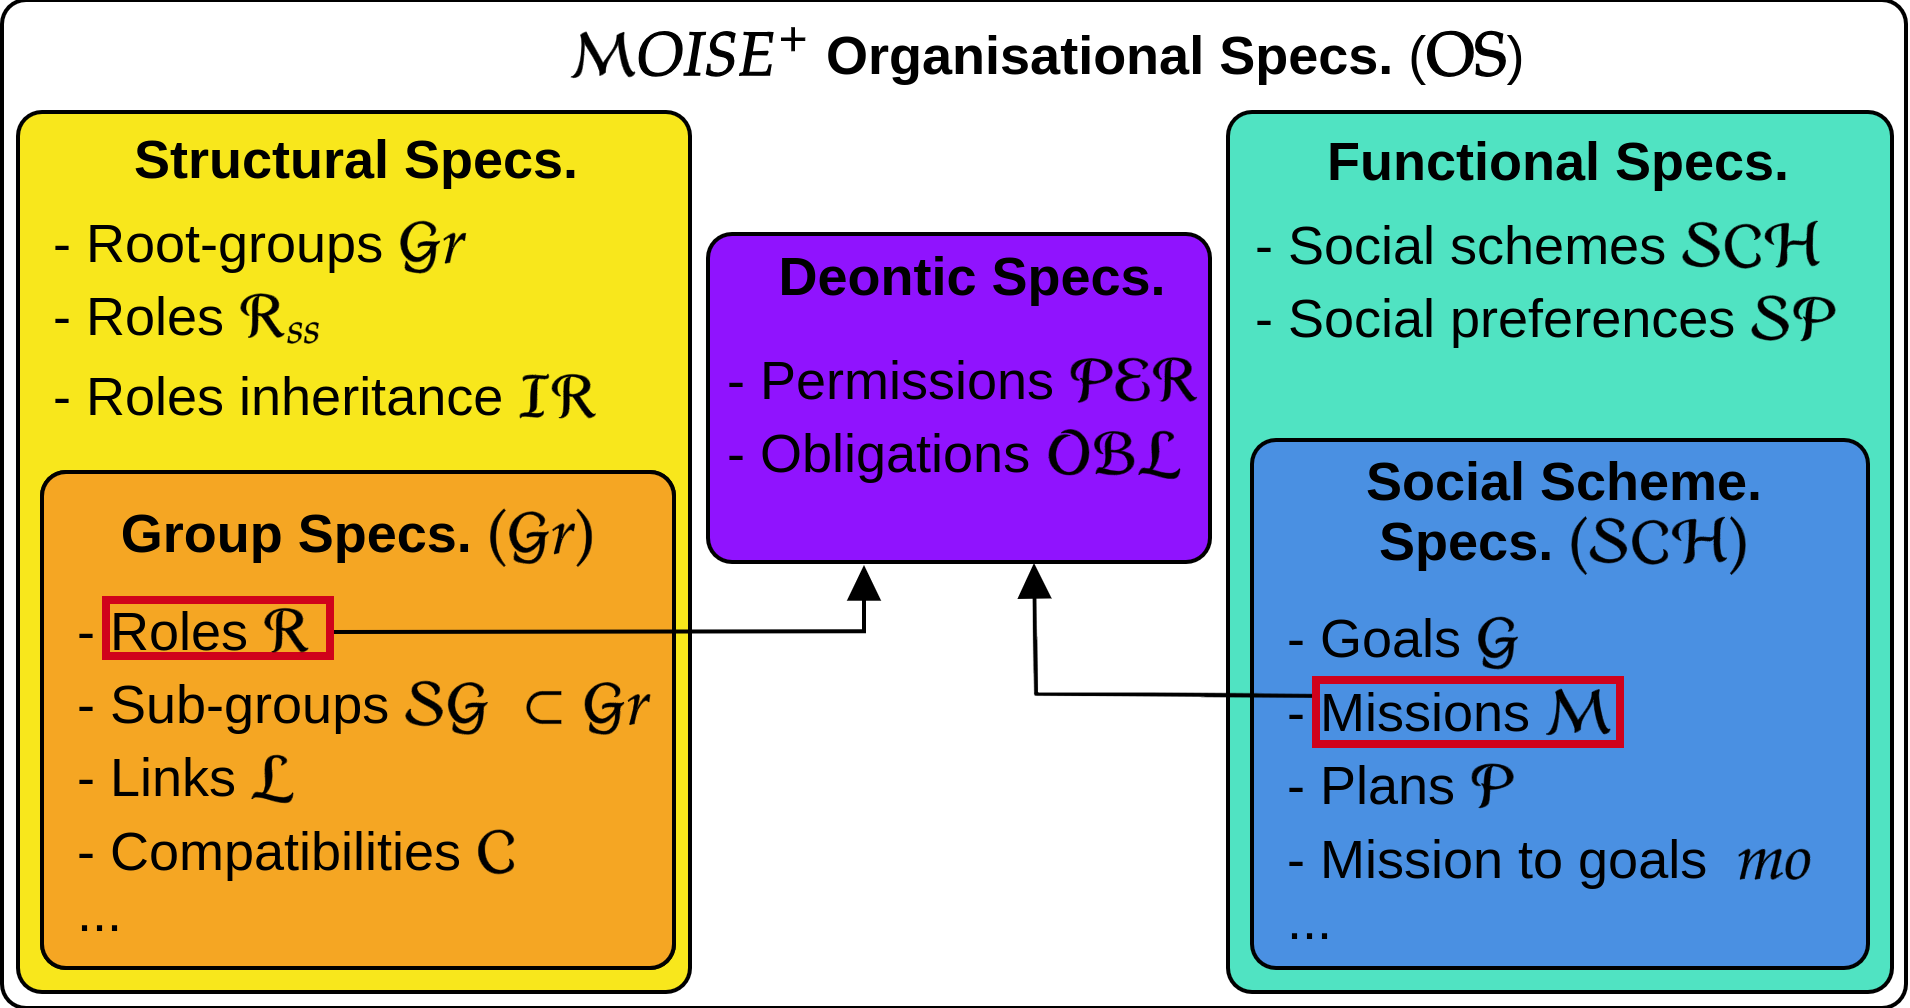
\includegraphics[width=0.9\linewidth]{figures/moise_model.png}
    \end{figure}

\end{frame}

\begin{frame}{Theoretical background}{Organizational model: \textit{soccer team example}}

    \vspace{-4ex}
    \begin{figure}
        \centering
        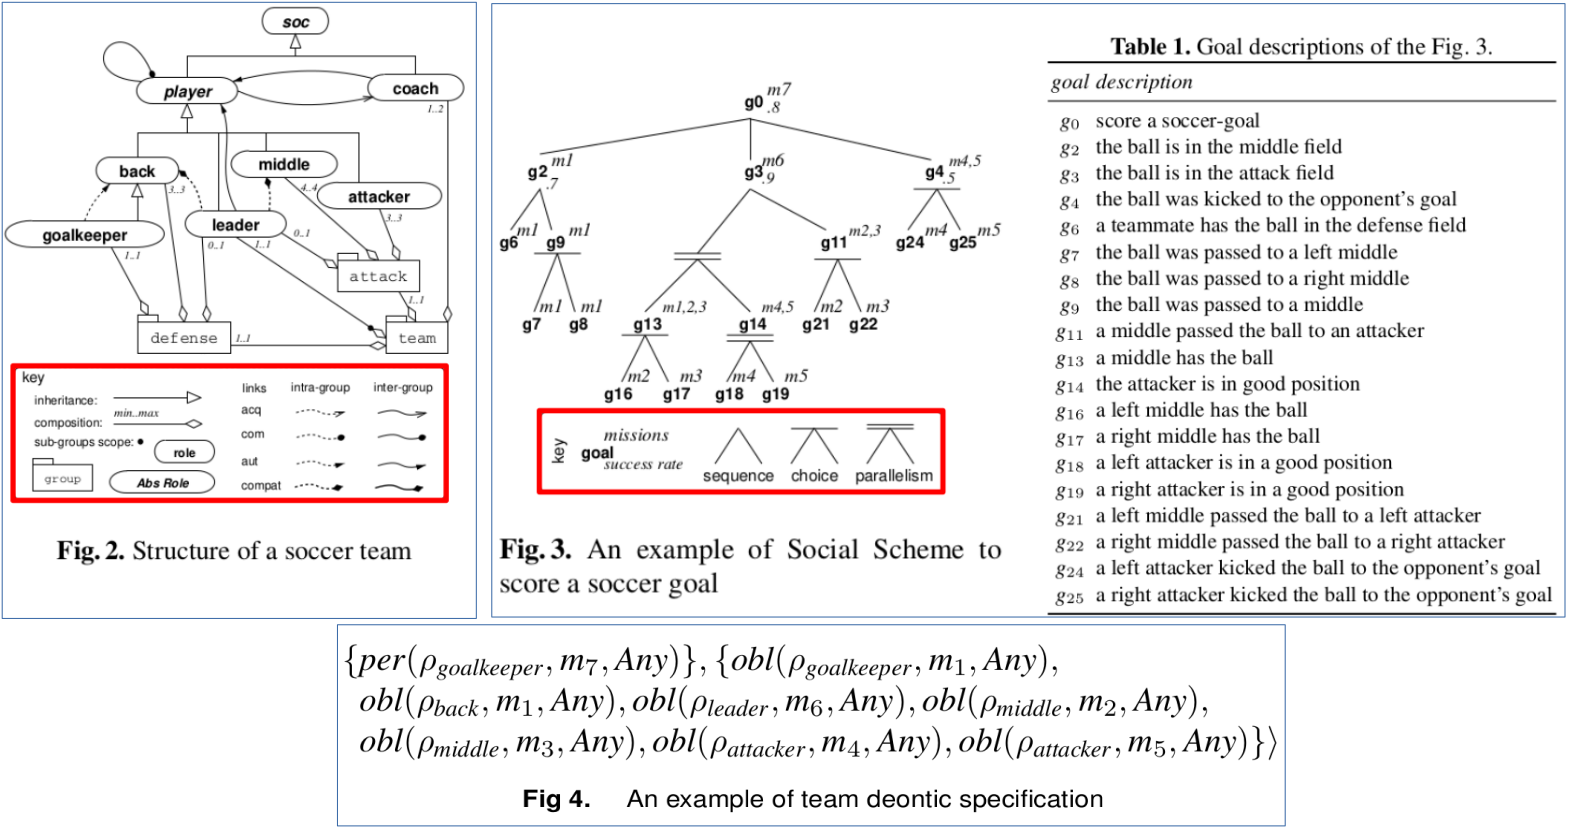
\includegraphics[width=0.85\linewidth]{figures/soccer_os.png}
    \end{figure}

    \begin{spacing}{0.25}
        {\tiny Hübner, J. F., Sichman, J. S., and Boissier, O. (2002).
            A model for the structural, functional, and deontic specification of
            organizations in multiagent systems.
            In Bittencourt, G. and Ramalho, G. L., editors, Proceedings of the 16th Brazilian Symposium on Artificial Intelligence (SBIA’02), volume 2507 of LNAI, pages 118–128, Berlin. Springer.}
    \end{spacing}


\end{frame}


\subsection{MARL basics}

\begin{frame}{Theoretical background}{MARL basics}

    \begin{columns}

        \hspace{-2ex}

        \begin{column}{0.4\textwidth}

            \begin{figure}
                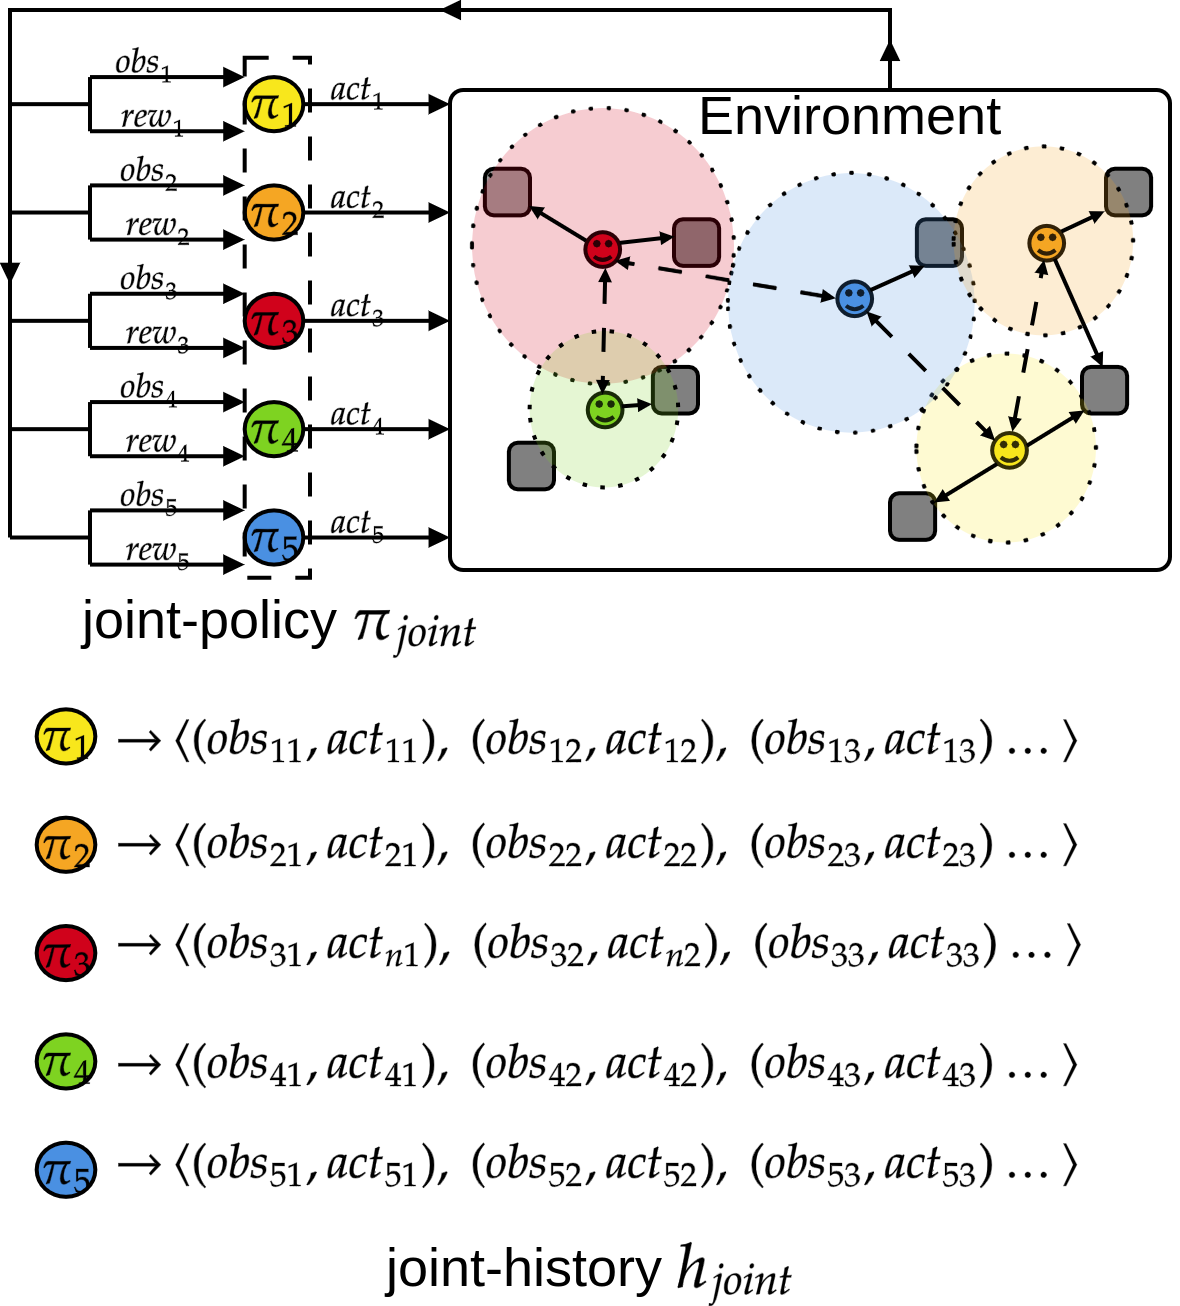
\includegraphics[width=\linewidth]{figures/marl_basics.png}
            \end{figure}

        \end{column}

        \begin{column}{0.7\textwidth}

            \begin{block}{Markovian models for MARL: Dec-POMDP}
                Decentralized Partially Observable Markov Decision Process~\cite{Oliehoek2016}
                \begin{itemize}
                    \item considers multiple agents in a similar MAS fashion
                    \item stochastic processes for uncertainty in environmental changes including observations;
                    \item reward function is common to agents which fosters training for collaborative oriented actions~\cite{Beynier2013}
                \end{itemize}

                \

                { \scriptsize

                $(S,\{A_i\},T,R,\{\Omega_i\},O,\gamma)$ , where
                \begin{itemize}
                    \item $S = \{s_1, ..s_{|S|}\}$: The set of the possible states;
                    \item $A_{i} = \{a_{1}^{i},..,a_{|A_{i}|}^{i}\}$: The set of the possible actions for agent $i$;
                    \item $T$ so that $T(s,a,s') = \probP{(s'|s,a)}$ : The set of conditional transition probabilities between states;
                    \item $R: S \times A \times S \rightarrow \mathbb{R}$: The reward function
                    \item $\Omega_{i} = \{o_{1}^{i},..,o_{|\Omega_{i}|}^{i}\}$: The set of observations for agent $ag_i$;
                    \item $O$ so that $O(s',a,o) = \probP{(o|s',a)}$ : The set of conditional observation probabilities;
                    \item $\gamma \in [0,1]$, the discount factor.
                \end{itemize}

                }

            \end{block}

        \end{column}

    \end{columns}

\end{frame}

\begin{frame}{Theoretical background}{MARL for solving/designing}

    \begin{block}{MARL for methodological purpose in literature?}

        Effective joint-policies but \textbf{not explicitly} specified/understandable
        $\Longrightarrow$ Few related works
            {\small
                \begin{itemize}
                    \item Kazhdan et. al.~\cite{Kazhdan2020} proposed means to extract symbolic models;
                    \item Wang et. al.~\cite{Wang2020}: introduced a role-oriented MARL approach;
                    \item Zheng et. al.~\cite{Zheng2018} presented a platform for MARL.
                \end{itemize}
            }
    \end{block}

    \begin{block}{Solving a Dec-POMDP}
        \begin{itemize}
            \item \textbf{solving}: finding a joint policy $\pi_{joint,i} \in \Pi_{joint}$ maximizing cumulative reward over time;
            \item \textbf{sub-optimally solving}: finding a joint policy $\pi_{joint,i} \in \Pi_{joint}$ so that expected cumulative reward over time at least at $s \in \mathbb{R}$.
        \end{itemize}
    \end{block}

    \begin{exampleblock}{Examples of MARL Algorithms}
        {\footnotesize

            \centering
            \begin{minipage}{0.5\textwidth}
                \centering
                \begin{itemize}
                    \item \textbf{Independent Learning}: IQL, IDQN
                    \item \textbf{Centralized Training, Decentralized Execution}: MADDPG, COMA, VDN
                \end{itemize}
            \end{minipage}\hfill
            \begin{minipage}{0.5\textwidth}
                \centering
                \begin{itemize}
                    \item \textbf{Cooperative MARL}: QMIX, MAPPO
                    \item \textbf{Hierarchical MARL}: Feudal Networks, Hierarchical Actor-Critic
                \end{itemize}
            \end{minipage}\hfill
        }
    \end{exampleblock}

\end{frame}
